\documentclass[12pt]{article}
\setlength{\parindent}{0in}
\setlength{\parskip}{\baselineskip}

\usepackage[top=0.75in, bottom=0.75in, left=1in, right=1in]{geometry}

\usepackage{amsmath,amsfonts,amssymb,graphicx, hyperref, float}

\begin{document}

IBEHS 4A03 \hfill Assignment \#3\\
Baoze Lin, Hady Ibrahim

\hrulefill

% Custom numbering for subparts (e.g., 2.1, 2.2)
\renewcommand{\theenumii}{\arabic{enumi}.\arabic{enumii}}

\begin{enumerate}
\item Question 1
  \begin{enumerate}
    % Answer to 1.1
    \item
    Blah Blah Figure \ref{fig:figure1_1}
    
    \begin{figure}[H]
      \centering
      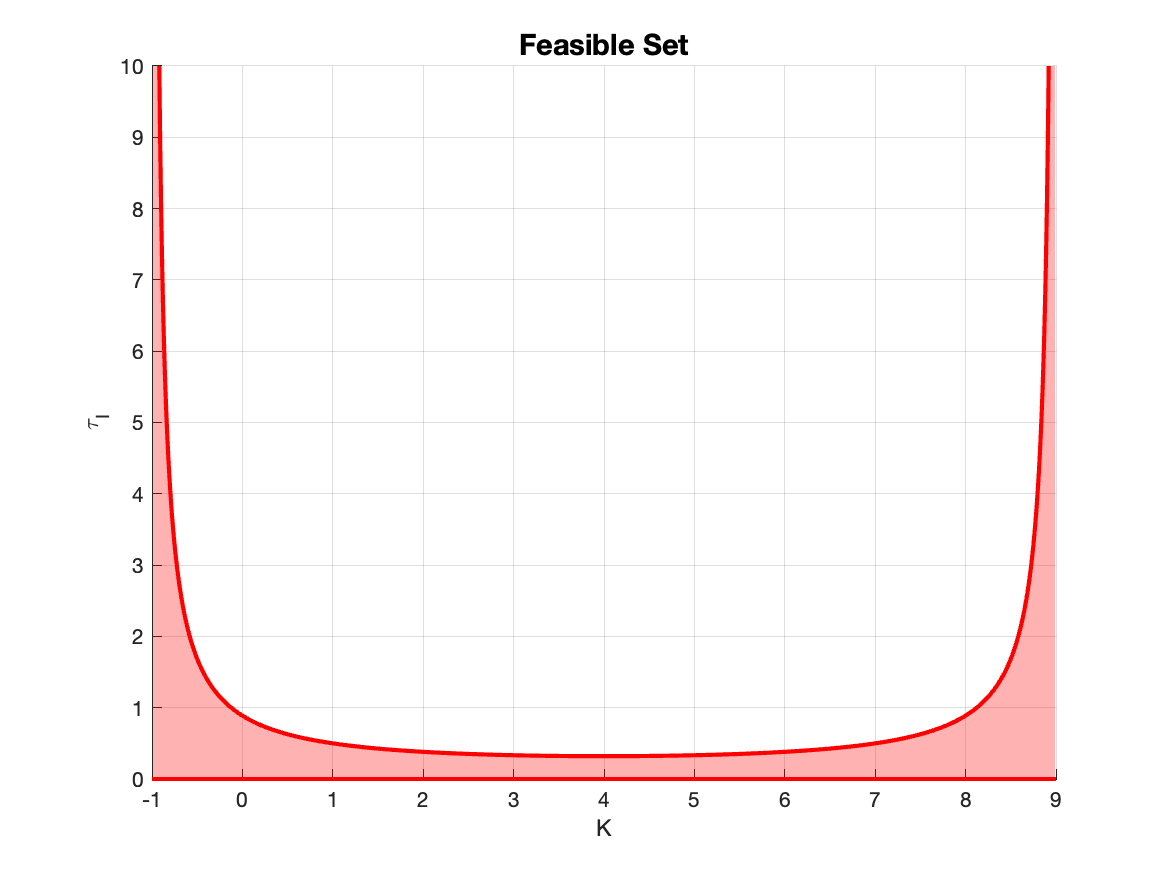
\includegraphics[width=0.3\textwidth]{Figures/figure1-2a.png}
      \caption{Simulink model of the open-loop step response}
      \label{fig:figure1_1}
    \end{figure}

    % Answer to 1.2
    \item hfill
    
    % Answer to 1.3
    \item hfill
    
    For the on the edge response, it is hard to see but the response is slowly oscillating larger and larger (VERY SLOWLY). It is unstable, but only seen over a long period of time. This is because for our conditions, we calculated that the values must be $>$ the drawn curved line. Picking values $=$ to that line still causes instability.

  \end{enumerate}

\clearpage
\item Question 2
  \begin{enumerate}
    % 2.1
    \item Write answer here
     
  \end{enumerate}

\end{enumerate}

\end{document}
